\title{OpenMPI and parallel Shift-Dictionary with Doublestep calculation}
\date{\today}

\documentclass[12pt]{article}

\usepackage{amsmath}
\usepackage{algorithm}
\usepackage[noend]{algpseudocode}
\usepackage{tikz}
\usepackage{graphicx}
\graphicspath{ {./images/} }

\makeatletter
\def\BState{\State\hskip-\ALG@thistlm}
\makeatother


\begin{document}
\maketitle

\section{Problem}
Our current algorithms tries to handle the addition of multiple visibilites at once. To achieve this, we group all visibilities together, that have the same shift-index. For every one of these groups we calculate the shift-vector that is representative of all visibilities in this group and. This is simply the sum of all shift-vectors in this group.
Threw modeling we have seen, that in most cases we need N groups, since every shift-index appears at least once, in visibility-clusters of relevant size. We usually store the shift-vectors of all groups in a dictionary. I will call this the shift-dictionary. After that we will use the double-step algorithms described in the next section to update the sub-grids of the image-matrix. Because of the way Doublestep works, it will be more efficient to calculate all shift-vectors with column-shift first and process, and then handle all row-shiftable shift-vectors. \\

Using our current implementation of Spift with Apache-Flink, we calculate the shift-dictionary in every parallel task and then every task then updates its sub-grid (Figure \ref{fig:floatSPIFT}). We present hear an idea to calculate the shift-dictionary in parallel, and then use a method we call double-shift to get ride of redundant complex-additions when calculating the sub-grids. \\

\begin{figure}
\resizebox{100mm}{50mm}{

\begin{tikzpicture}[node distance={30mm}, main/.style = {draw, rectangle}, transform shape] 
\node[main] (1) {StreamSource};
\node[main] (2) [right of=1]{isRowShift};
\node[main] (3) [right of=2]{shiftIndex};
\node[main] (4) [right of=3]{partition};

\node[main] (7) [above right of=4]{shif-dic};
\node[main] (8) [right of=7]{set-subGrid2};
\node[main] (5) [above of=7]{shift-dic};
\node[main] (6) [right of=5]{set-subGrid1};
\node[main] (9) [below right of=4]{shif-dic};
\node[main] (10) [right of=9]{set-subGrid3};
\node[main] (11) [below of=9]{shift-dic};
\node[main] (12) [right of=11]{set-subGrid4};
\node[main] (13) [below right of=8]{output-stream};

\draw (1)--(2);
§\draw (2)--(3);
\draw (3)--(4);
\draw (4)--(5); \draw (5)--(6);  \draw (6)--(13);
\draw (4)--(7); \draw (7)--(8);  \draw (8)--(13);
\draw (4)--(9); \draw (9)--(10);  \draw (10)--(13);
\draw (4)--(11); \draw (11)--(12);  \draw (12)--(13);


\end{tikzpicture} 

}

\caption{Flowchart SPIFT}
\label{fig:floatSPIFT}
\end{figure}

\section{General Idea}

We propose to calculate the shift-dictionary only once per machine,and use the parallel Doublestep-algorithm we developed using all processes available on one machine. Parallel processes on the same machine could use shared memory for fast access (Figure \ref{fig:floatDOUBLE}). As long as the processes only share information on the same machine, the communication overhead should be acceptable.\\

We could not find a way to do this in Apache-Flink. Flink handles the distribution of processes to machines internally and treats all processes the same, independent of where they are running. So communication of nodes on the same machine is not intended and not supported. So we propose to use OpenMPI and C (or C++). OpenMPI can handle communication between different machines, but it will also allow shared Memory between processes on the same machine.\\

With this new system, new variables get relevant. The amount of physical machines we call $mp$, the amount of local processes on machine $i$ we call $lp_i$ and the amount of processes on all machines combined we call $gp$.

\begin{figure}
\resizebox{100mm}{50mm}{

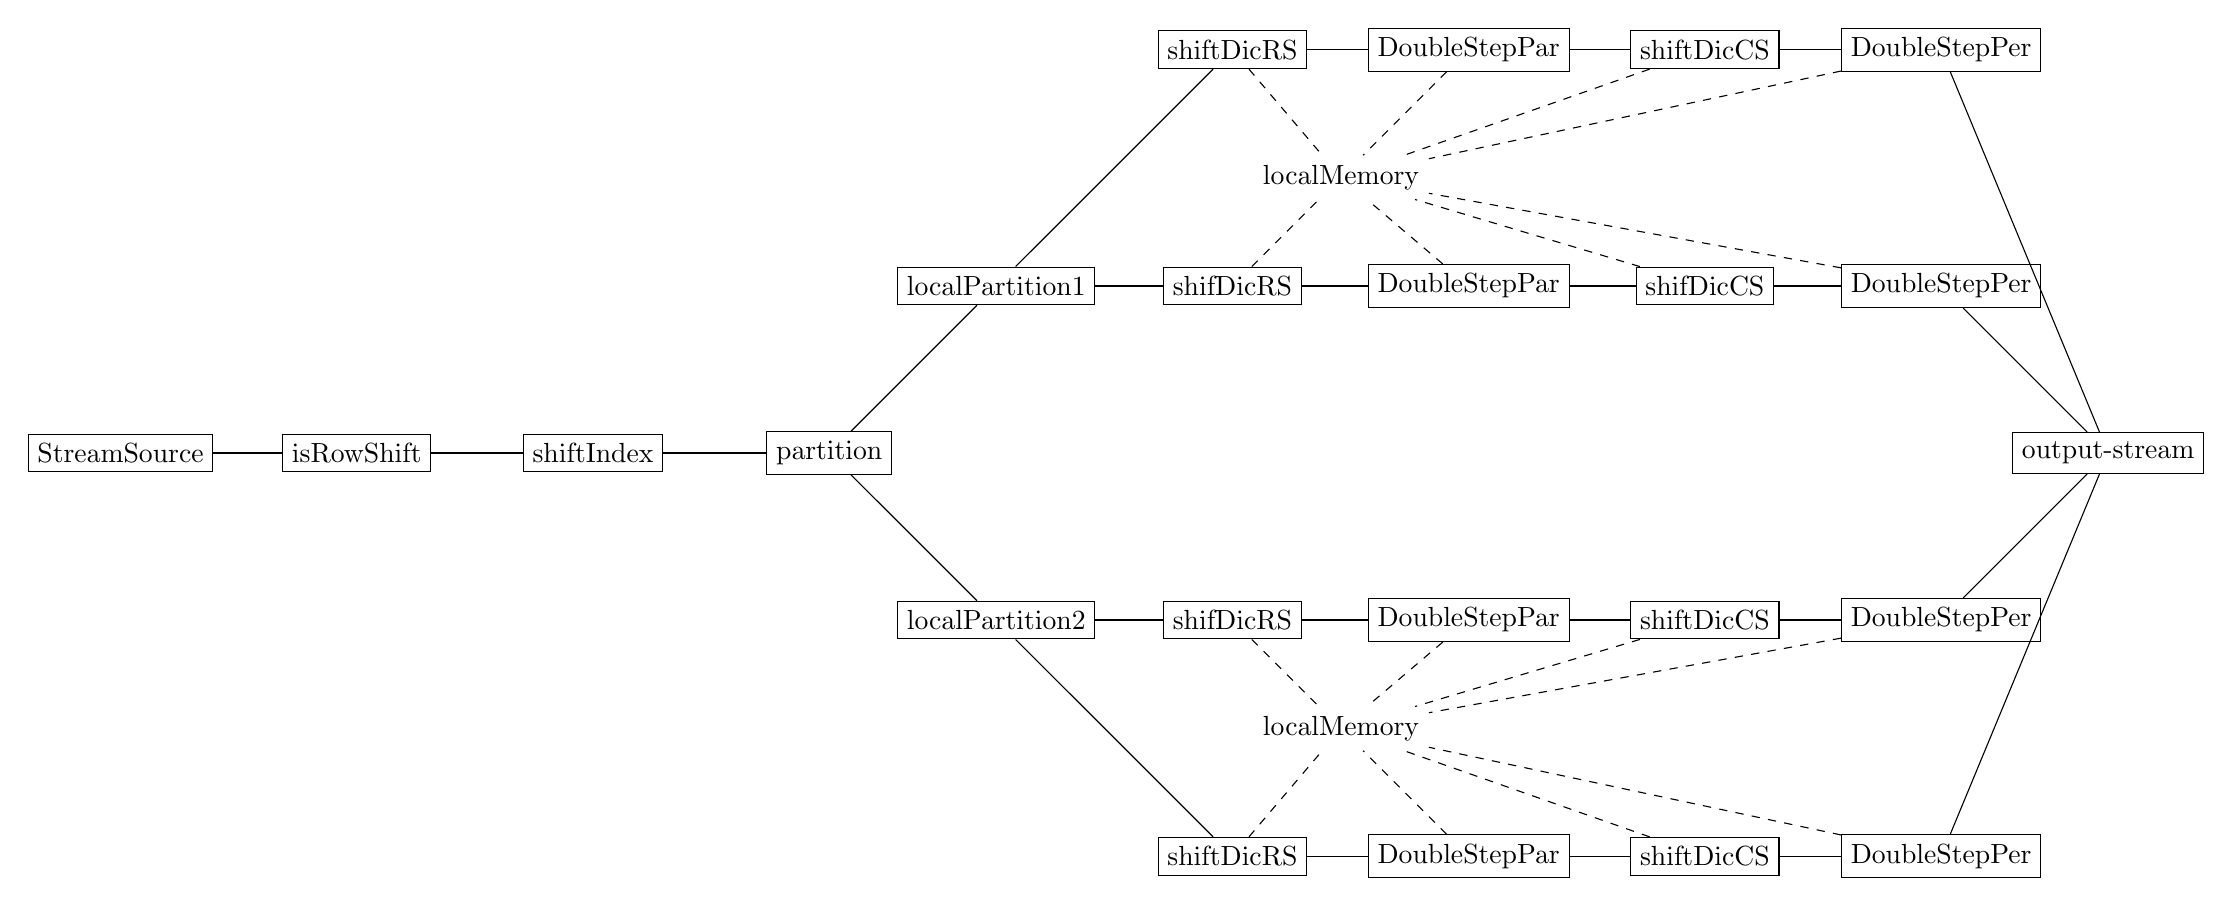
\begin{tikzpicture}[node distance={30mm}, main/.style = {draw, rectangle}, transform shape] 
\node[main] (1) {StreamSource};
\node[main] (2) [right of=1]{isRowShift};
\node[main] (3) [right of=2]{shiftIndex};
\node[main] (4) [right of=3]{partition};

\node[main] (lp1) [above right of=4]{localPartition1};
\node[main] (9) [right of=lp1]{shifDicRS};
\node[main] (10) [right of=9]{DoubleStepPar};
\node[main] (11) [right of=10]{shifDicCS};
\node[main] (12) [right of=11]{DoubleStepPer};

\node[main] (5) [above of=9]{shiftDicRS};
\node[main] (6) [right of=5]{DoubleStepPar};
\node[main] (7) [right of=6]{shiftDicCS};
\node[main] (8) [right of=7]{DoubleStepPer};

\node[main] (lp2) [below right of=4]{localPartition2};
\node[main] (13) [right of=lp2]{shifDicRS};
\node[main] (14) [right of=13]{DoubleStepPar};
\node[main] (15) [right of=14]{shiftDicCS};
\node[main] (16) [right of=15]{DoubleStepPer};

\node[main] (17) [below of=13]{shiftDicRS};
\node[main] (18) [right of=17]{DoubleStepPar};
\node[main] (19) [right of=18]{shiftDicCS};
\node[main] (20) [right of=19]{DoubleStepPer};

\node[main] (os) [below right of=12]{output-stream};

\node at(15.5,3.5) (sm1) {localMemory};
\node at(15.5,-3.5) (sm2) {localMemory};


\draw (1)--(2);
\draw (2)--(3);
\draw (3)--(4);
\draw (4)--(lp1);
\draw (lp1)--(5); \draw (5)-- (6);  \draw (6)-- (7); \draw (7)-- (8); \draw (8)--(os);
\draw (lp1)--(9); \draw (9)--(10);  \draw (10)-- (11); \draw (11)-- (12); \draw (12)--(os);

\draw (4)--(lp2);
\draw (lp2)--(13); \draw (13)--(14);  \draw (14)--(15); \draw (15)--(16); \draw (16)--(os);
\draw (lp2)--(17); \draw (17)--(18);  \draw (18)--(19); \draw (19)--(20); \draw(20)--(os);

\draw (5)--(sm1)[dashed]; \draw (6)--(sm1)[dashed]; \draw (7)--(sm1)[dashed]; \draw (8)--(sm1)[dashed];
\draw (9)--(sm1)[dashed]; \draw (10)--(sm1)[dashed]; \draw (11)--(sm1)[dashed]; \draw (12)--(sm1)[dashed];
\draw (13)--(sm2)[dashed]; \draw (14)--(sm2)[dashed]; \draw (15)--(sm2)[dashed]; \draw (16)--(sm2)[dashed];
\draw (17)--(sm2)[dashed]; \draw (18)--(sm2)[dashed];  \draw (19)--(sm2)[dashed];  \draw (20)--(sm2)[dashed];


\end{tikzpicture} 

}

\caption{Flowchart SPIFT with shared memory and Doublestep}
\label{fig:floatDOUBLE}
\end{figure}

\section{ Doublestep }

The naive approach of calculating the final matrix is to add all the shifted values for every entry of the matrix. This leads to a lot of additions getting done multiple times. We developed the double-step algorithm to insure every addition only happens once.

\subsection{ Simple Doublestep }

Consider two shift-vectors $\vec{v}_1$ and $\vec{v}_2$ with shift-index $s_1$ and $s_2$ where $s_1 = s_2+\frac{N}{2}$ which are both row-shiftable. In the first row, $\vec{v}_1$ and $\vec{v}_2$ get added together $\vec{v}_1[0]+\vec{v}_2[0]$ ([*] denotes by how much the vector is shifted). On the next row, we get $\vec{v}_1[s_1]+\vec{v}_2[s_2]$. On the third row, it's $\vec{v}_1[2*s_1]+\vec{v}_2[2*s_2] = \vec{v}_1[2*s_1]+\vec{v}_2[2*s_1+2*\frac{N}{2}] = \vec{v}_1[2*s_1]+\vec{v}_2[2*s_1] = (\vec{v}_1[0]+\vec{v}_2[0])[2*s_1] $. And on the forth $\vec{v}_1[4*s_1]+\vec{v}_2[4*s_2] = (\vec{v}_1[s_1]+\vec{v}_2[s_1 +\frac{N}{2}])[2*s_1]$.\\

As we can see, we only need to make two vector-additions, $\vec{v}_1[0]+\vec{v}_2[0]$ and $\vec{v}_1[s_1]+\vec{v}_2[s_2]$. These two rows form a $2\times N$-matrix. If we shift this matrix by a multiple of $2*s_1$, it corresponds to the shifted addition of $v_1$ and $v_2$. We will call this matrix $sm_{2*s_1}^2$, where the subscript denotes the shift-index of the shift-matrix, and the superscript denotes the amount of rows it has. We can do this with all shift-vector-pairs to get $\frac{N}{2}$ shift-matrices, that all have an even shift-index.\\

Using all the $2\times N$-shift-matrices, we can use the same method to construct $\frac{N}{4}$ $4\times N$-matrices with shift-vectors that are multiple of four. We repeat this process until we have calculated $sm_{0}^N$, which is the final matrix. Figure \ref{fig:DS} shows the process on a $8\times 8$ matrix with row-shifted vectors.

\begin{figure}[h!]
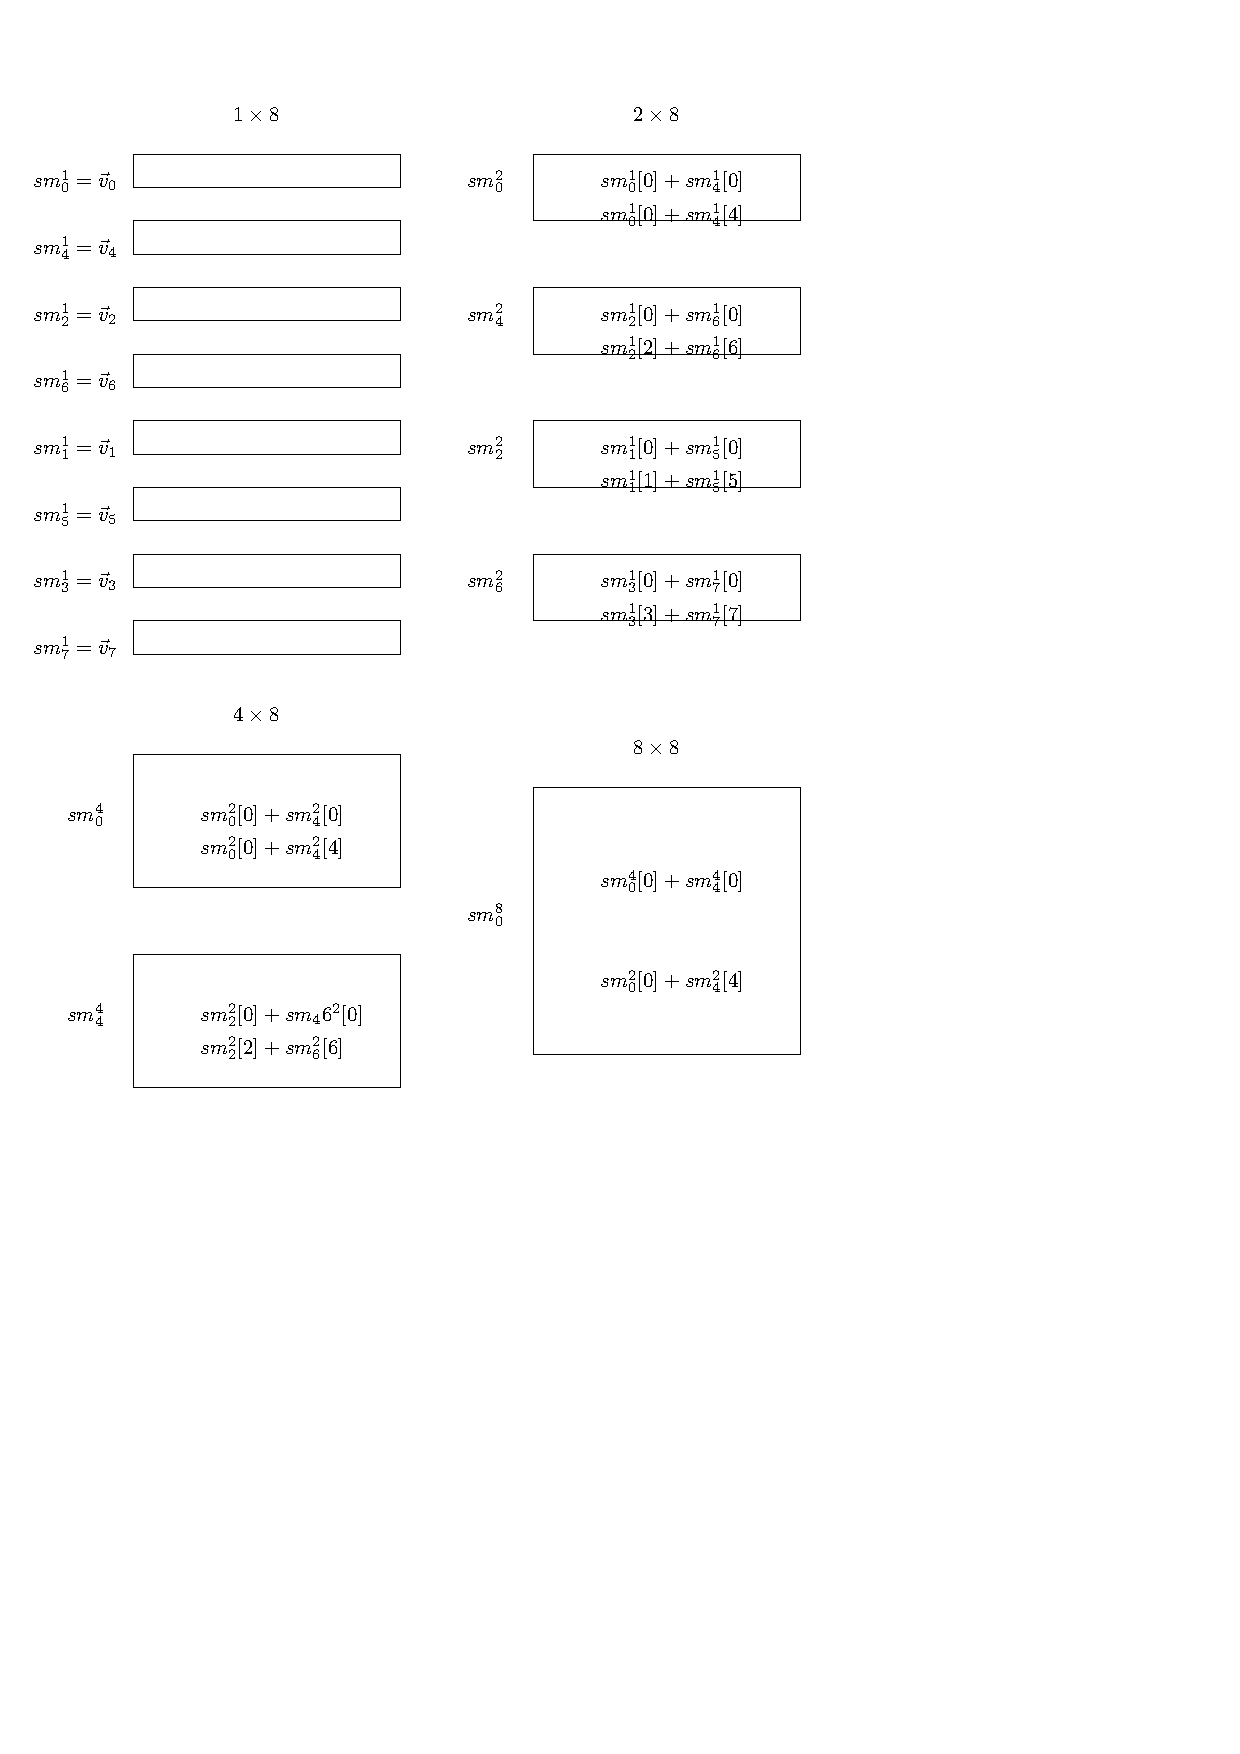
\includegraphics[scale=0.7]{Doublestep_overview}
\caption{example Doublestep}
\label{fig:DS}
\end{figure}

\subsection{ Parallel-computed Doublestep }

In our case, multiple processes work together to calculate a sub-grid of the image matrix. Since how the image-matrix is sliced is fixed, we get two different cases. In one case, the slicing is parallel to the shift-type (e.g. row shift and row slice). In this case only a few steps of Doublestep need to be calculated. Figure \ref{fig:DSparallel} shows how to do this, if only the red part needs to be calculated. \\


\begin{figure}
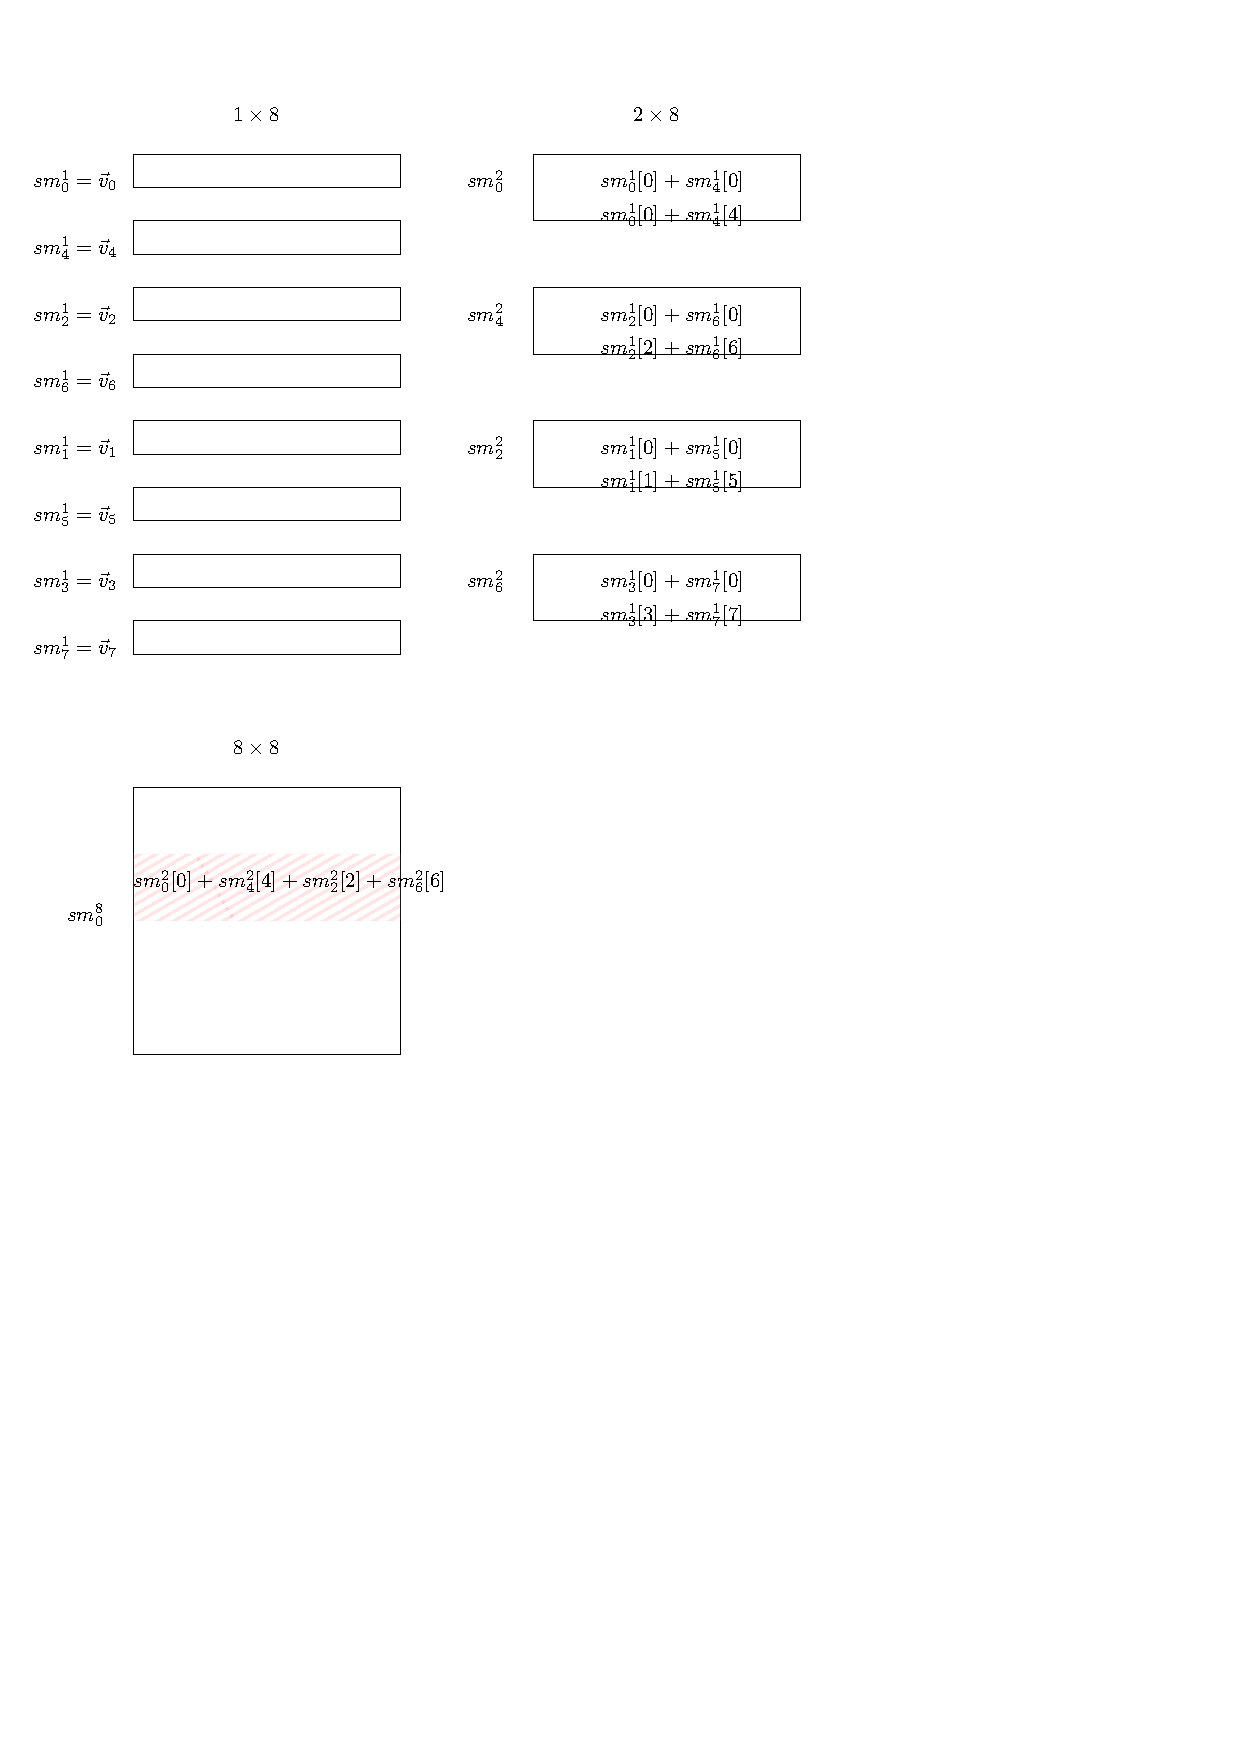
\includegraphics[scale=0.7]{Doublestep_parallel}
\caption{Doublestep parallel}
\label{fig:DSparallel}
\end{figure}

When the slicing is parallel to the shift (e.g. column shift and row slice), all steps of Doublestep need to be calculated. But since only a sub grid of the image matrix is needed, only certain lines need to be calculated. This is shown in Figure \ref{fig:DSperpendicular}. The red shows the values that need to be calculated.


\begin{figure}
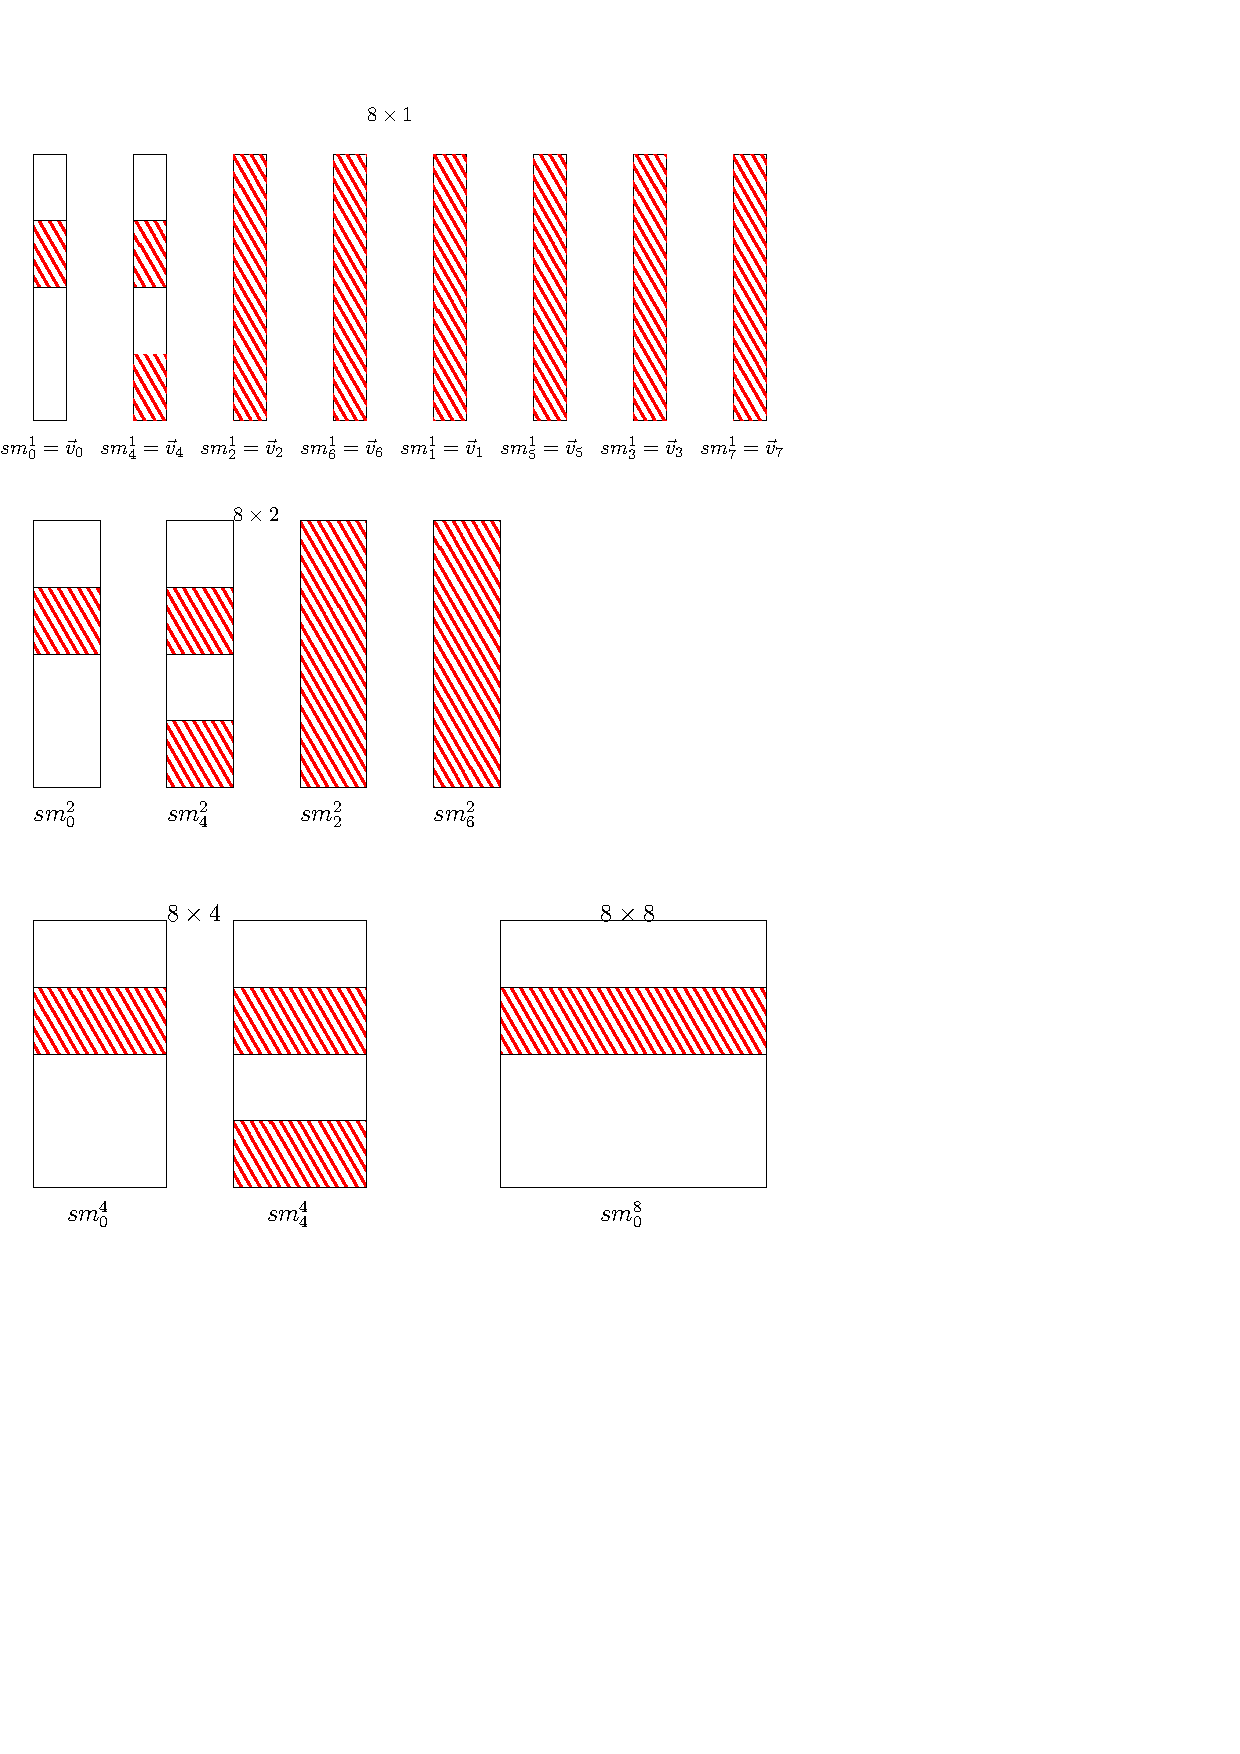
\includegraphics[scale=0.7]{Doublestep_perpendicular}
\caption{Doublestep parallel}
\label{fig:DSperpendicular}
\end{figure}

\section{ Comparisons }

Table \ref{table:comp} compares the naive approach with Doublestep using OpenMPI. $lp_i$ denotes the amount of local processes on machine $i$, and $D_i=\frac{N*lp_i}{gp}$ the amount of lines that the sub-grid calculated by machine $i$ has. In all cases where $lp_i>1$, the system we propose would require less memory, and in all cases it would be faster than the current approach.

\begin{table}
\label{table:comp}
\begin{tabular}{ |c|c|c| }
 \hline
  & Memory-needs & Complexity \\ 
 Naive & $N^2*lp_i$ & $\mathcal{O}(\frac{N^3}{lp_i})$ \\ 
 Double Step and OpenMPI &  $2*\frac{N^2}{lp_i}$ & $\mathcal{O}(\frac{N^2*log(D_i)}{lp_i}) )$\\ 
 \hline
\end{tabular}
\caption{compare deficiencies}
\end{table}

\end{document}
